\subsection{Anpassungen in der SPS}

Nach der Implementierung der Auftragssteuerung musste sichergestellt werden, dass der Auslagerprozess mit dem entwickelten Python-Softwarekonzept synchronisiert wird.\\
Um diese Integration zu realisieren, wurden sowohl software- als auch hardwareseitige Anpassungen innerhalb der SPS vorgenommen.
\subsubsection{Datenbausteine im Kontext der auftragsbasierten Auslagerung}

Das vorliegende System umfasst bereits grundlegende Prozessschrittketten für die Funktionen Einlagern, Auslagern und Umlagern. 
Eine detaillierte Beschreibung dieser Abläufe ist in der Dokumentation der Studienarbeit T3\_3100 enthalten.\\

Für die Kommunikation zwischen der externen Programmanwendung und der \textbf{SPS} wurde ein zusätzlicher Datenbaustein implementiert. Dieser ermöglicht einen strukturierten Datenaustausch über die Snap7-Schnittstelle.\\

Grundsätzlich erfolgt der Zugriff über Snap7 durch direkte Adressierung von Variablen anhand der Datenbaustein-Nummer sowie der zugehörigen Speicheradressen.

\begin{figure}[H]
	\centering
	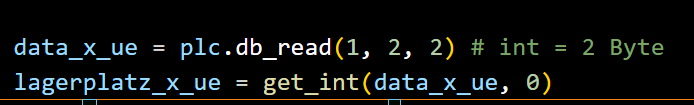
\includegraphics[width=0.8\textwidth]{Screenshots/Auftragsbasierte Auslagerung/snap7.png}
	\caption{Einlesen einer Variablen aus der SPS mittels Snap7}
	\label{fig:Snap7_Einlesen}
\end{figure}

In Abbildung \ref{fig:Snap7_Einlesen} ist ein beispielhafter Einlesevorgang dargestellt. Die Funktion \texttt{db\_read} ermöglicht den Zugriff auf eine Variable innerhalb eines Datenbausteins, in diesem Fall auf \texttt{Lagerplatz\_x\_ue}.\\

Die übergebenen Parameter definieren dabei die Datenbaustein-Nummer, die Startadresse im Speicher sowie die Größe des auszulesenden Datentyps. Für einen \textbf{Integer} werden standardmäßig 2 Byte verwendet. Für andere Datentypen muss die entsprechende Größe angepasst werden.\\

Nach diesem Prinzip werden alle erforderlichen Informationen, wie beispielsweise Lagerplatz- oder Artikelnummern, aus den bestehenden Datenbausteinen ausgelesen und in der Programmanwendung weiterverarbeitet.\\

Für die Realisierung eines zuverlässigen \textbf{Handshakes} zwischen \textbf{SPS} und Python-Anwendung wurden zusätzliche Signale eingeführt. Hierzu wurde ein weiterer Datenbaustein angelegt, der speziell der Kommunikation dient.\\

Um einen direkten Zugriff auf die Speicheradressen zu ermöglichen, wurde der \textbf{optimierte Bausteinzugriff} deaktiviert. Nach dieser Anpassung musste der Datenbaustein neu übersetzt werden, um eine korrekte Adressierung zu gewährleisten.

\begin{figure}[H]
	\centering
	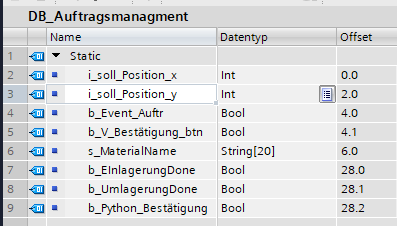
\includegraphics[width=0.8\textwidth]{Screenshots/Auftragsbasierte Auslagerung/TIA_DB41.png}
	\caption{Datenbaustein für das Auftragsmanagement}
	\label{fig:DB_Auftrag}
\end{figure}

In Abbildung \ref{fig:DB_Auftrag} sind die neu eingeführten Variablen mit ihren jeweiligen Adressen dargestellt.\\
Die Variablen \texttt{i\_Soll\_Position} sowie \texttt{s\_MaterialName} werden durch die Python-Anwendung gesetzt und enthalten die relevanten Informationen für den Auslagerprozess, wie beispielsweise Artikelnummer und Lagerplatzkoordinaten.\\
Zusätzlich wurden Steuer- und Statussignale wie \texttt{b\_EinlagerungDone}, \texttt{b\_UmlagerungDone} sowie \texttt{b\_Python\_Bestaetigung} eingeführt. Diese dienen der Umsetzung eines zuverlässigen Handshakes und gewährleisten, dass die Daten nach jedem Ein- oder Umlagerprozess korrekt verarbeitet und synchronisiert werden.\\

Die Variable \texttt{b\_Event\_Auftr} ermöglicht der SPS das Erkennen eines neuen Auftrags. Über die Variable \texttt{b\_V\_Bestaetigung\_btn} kann ein Bestätigungssignal vom \textbf{HMI} verarbeitet werden, welches den Start des Auslagerprozesses auslöst.\\

Nach der Implementierung des Datenbausteins konnte im nächsten Schritt die Anpassung der Prozessschrittkette erfolgen.

\subsubsection{Anpassung der Prozessschrittkette ``Auslagern''}
Im vorherigen Abschnitt wurden die neu eingeführten Variablen bereits erläutert. Im Folgenden wird die Anpassung der Prozessschrittkette ``Auslagern'' innerhalb der SPS beschrieben.\\

Im ursprünglichen System wurde der Auslagerprozess manuell über einen Button im \textbf{HMI} gestartet. Nach der Auslösung erfolgt innerhalb der SPS ein Soll-Ist-Vergleich der Ziel- und Ist-Positionen in X- und Y-Richtung. Anschließend wird das entsprechende Material aus dem Lager entnommen.\\

\begin{figure}[H]
	\centering
	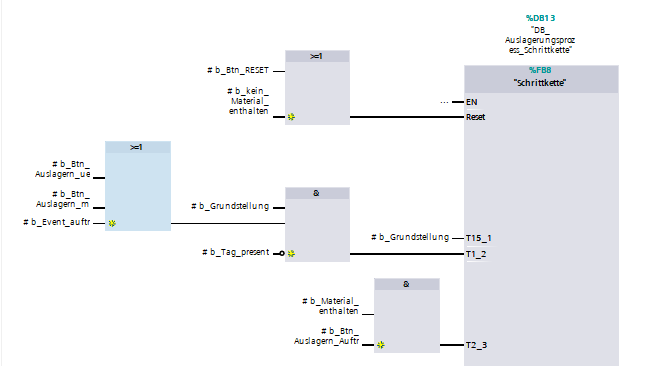
\includegraphics[width=0.8\textwidth]{Screenshots/Auftragsbasierte Auslagerung/TIA_Auslagerung.png}
	\caption{Prozessablauf der Auslagerung in der SPS}
	\label{fig:Auslagerung}
\end{figure}

Im Zuge der Erweiterung hin zu einer auftragsbasierten Steuerung wurde dieser Ablauf angepasst und um zusätzliche Prozessschritte ergänzt\ref{fig:Auslagerung}.\\

Zunächst wurde ein Triggermechanismus implementiert, bei dem die \textbf{SPS} den Scanner gezielt aktiviert.

\begin{figure}[H]
	\centering
	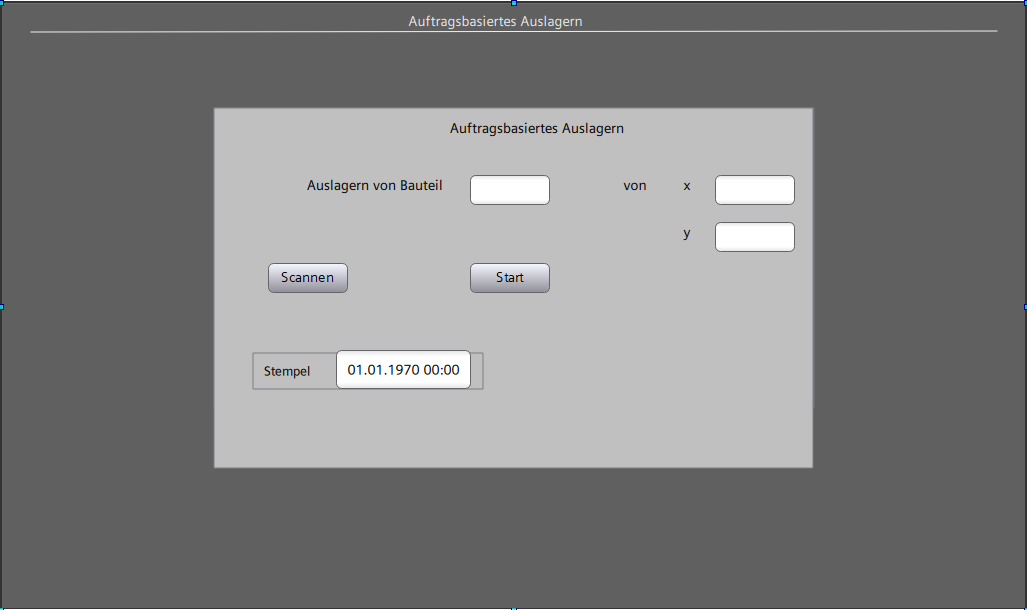
\includegraphics[width=0.8\textwidth]{Screenshots/Auftragsbasierte Auslagerung/HMI_Auftrag.png}
	\caption{Darstellung des auftragsbasierten Auslagerungsprozesses im HMI}
	\label{fig:AuftragHMI}
\end{figure}
Hierzu wird ein entsprechendes Signal gesetzt, wodurch der Scanner einen Scanvorgang ausführt und den erfassten Code an die Programmanwendung übergibt (vgl. Abbildung \ref{fig:AuftragHMI}).\\

Auf Basis dieses Codes erfolgt die Verarbeitung innerhalb der Programmanwendung. Die daraus resultierenden Steuerinformationen werden anschließend zurück an die SPS übertragen.\\

Zur eigentlichen Auslösung des Auslagerprozesses wurde die Variable \texttt{b\_Event\_Auftr} eingeführt. Diese wird durch die externe Programmanwendung gesetzt und signalisiert der SPS das Vorliegen eines neuen Auftrags.\\

Nach Erkennung dieses Signals wird der Prozess vorbereitet, jedoch noch nicht unmittelbar ausgeführt. Eine zusätzliche manuelle Freigabe durch den Bediener bleibt erforderlich. Diese erfolgt über das \textbf{HMI} mittels der Variable \texttt{b\_V\_Bestaetigung\_btn} (vgl. Abbildung \ref{fig:AuftragHMI}). Erst nach dieser Bestätigung wird der Auslagerprozess tatsächlich gestartet.\\

Durch diese Erweiterung konnte die bestehende Prozessschrittkette um eine auftragsbasierte Steuerung ergänzt werden. Gleichzeitig bleibt die Kontrolle über den Ablauf durch die manuelle Freigabe erhalten, wodurch die Betriebssicherheit der Anlage gewährleistet wird.